% =====================================================================
%  AI-Native AI Engineering -- Week 2 Project Instructions
%  A Probabilistic and Information-Theoretic View of AI Agents
%  ANTERN
%
%  Build:  tectonic main.tex
%      or: pdflatex main.tex  (run twice for the table of contents)
% =====================================================================
\documentclass[11pt,a4paper]{article}

% ---------- encoding and fonts ----------
\usepackage[T1]{fontenc}
\usepackage[utf8]{inputenc}
\usepackage{newtxtext,newtxmath}
\usepackage{microtype}

% ---------- layout ----------
\usepackage[margin=1in,headheight=14pt]{geometry}
\usepackage{fancyhdr}
\usepackage{titlesec}
\usepackage{enumitem}
\usepackage{parskip}

% ---------- tables, figures, colour ----------
\usepackage{booktabs}
\usepackage{array}
\usepackage{tabularx}
\usepackage{longtable}
\usepackage{multirow}
\usepackage{xcolor}
\usepackage{tikz}
\usetikzlibrary{arrows.meta,positioning,shapes.geometric,fit,backgrounds}
\let\Bbbk\relax
\usepackage{amsmath,amssymb}
\usepackage[framemethod=TikZ]{mdframed}
\usepackage{caption}

% ---------- links ----------
\usepackage[colorlinks=true,linkcolor=sblink,urlcolor=sblink,citecolor=sblink]{hyperref}

% ---------- palette ----------
\definecolor{sbink}{HTML}{1A1A1A}
\definecolor{sblink}{HTML}{0B4F6C}
\definecolor{sbrule}{HTML}{B3B3B3}
\definecolor{sbbox}{HTML}{F4F6F8}
\definecolor{sbaccent}{HTML}{8C1D40}
\definecolor{sbsoft}{HTML}{5B6770}

\color{sbink}

% ---------- headers ----------
\pagestyle{fancy}
\fancyhf{}
\fancyhead[L]{\footnotesize\color{sbsoft}AI-Native AI Engineering}
\fancyhead[R]{\footnotesize\color{sbsoft}Week 2 -- Probabilistic View of AI Agents}
\fancyfoot[C]{\footnotesize\color{sbsoft}\thepage}
\renewcommand{\headrulewidth}{0.4pt}
\renewcommand{\headrule}{\hbox to\headwidth{\color{sbrule}\leaders\hrule height \headrulewidth\hfill}}

% ---------- section styling ----------
\titleformat{\section}
  {\normalfont\large\bfseries\color{sbink}}{\thesection}{0.8em}{}
\titleformat{\subsection}
  {\normalfont\normalsize\bfseries\color{sbink}}{\thesubsection}{0.7em}{}
\titleformat{\subsubsection}
  {\normalfont\normalsize\itshape\color{sbink}}{\thesubsubsection}{0.7em}{}
\titlespacing*{\section}{0pt}{18pt}{7pt}
\titlespacing*{\subsection}{0pt}{12pt}{5pt}

% ---------- callout boxes ----------
\newmdenv[
  backgroundcolor=sbbox,
  linecolor=sbrule,
  linewidth=0.5pt,
  roundcorner=2pt,
  innertopmargin=8pt,
  innerbottommargin=8pt,
  innerleftmargin=10pt,
  innerrightmargin=10pt,
  skipabove=10pt,
  skipbelow=10pt
]{sbbox}

\newmdenv[
  topline=false,bottomline=false,rightline=false,
  linecolor=sbaccent,
  linewidth=2pt,
  innerleftmargin=10pt,
  innerrightmargin=0pt,
  innertopmargin=2pt,
  innerbottommargin=2pt,
  skipabove=10pt,
  skipbelow=10pt
]{sbrule}

\newcommand{\keyword}[1]{\textbf{#1}}
\newcommand{\rs}{Rs.\,}
\newcommand{\boxtitle}[1]{{\bfseries #1}\par\vspace{2pt}}

% ---------- teaching markers ----------
\newcommand{\taught}{\hfill{\footnotesize\sffamily\color{sbaccent}[extend this yourself]}}
\newcommand{\extend}{\hfill{\footnotesize\sffamily\color{sbaccent}[extend this yourself]}}

% ---------- learning-prompt box ----------
\newenvironment{learnprompt}
  {\begin{sbbox}\boxtitle{Prompt --- paste this into ChatGPT, Claude, or Gemini}%
   \ttfamily\small\raggedright}
  {\end{sbbox}}

\captionsetup{font=small,labelfont=bf}
\setlist[itemize]{leftmargin=1.4em,itemsep=2pt,topsep=3pt}
\setlist[enumerate]{leftmargin=1.6em,itemsep=2pt,topsep=3pt}

\newcolumntype{L}[1]{>{\raggedright\arraybackslash}p{#1}}
\newcolumntype{C}[1]{>{\centering\arraybackslash}p{#1}}

\begin{document}

% =====================================================================
\begin{titlepage}
\thispagestyle{empty}
\vspace*{2.2cm}
\begin{center}
{\footnotesize\sffamily\color{sbsoft}\MakeUppercase{ANTERN \quad$\cdot$\quad AI-Native AI Engineering}}\\[0.25cm]
{\footnotesize\sffamily\color{sbsoft}\MakeUppercase{Week 2 Project Instructions}}\\[1.4cm]

{\color{sbrule}\rule{0.72\textwidth}{0.4pt}}\\[0.9cm]

{\LARGE\bfseries A Probabilistic and Information-Theoretic\\[0.25cm] View of AI Agents\par}
\vspace{0.7cm}
{\large\itshape How an agent decides what to believe,\\[0.15cm] what to ask, and when to act\par}

\vspace{0.8cm}
{\color{sbrule}\rule{0.72\textwidth}{0.4pt}}\\[1.4cm]

\begin{minipage}{0.78\textwidth}
\small
\textbf{What this document is.} This is the Week 2 project brief. It extends the Week 1 project.
You keep the same problem. You keep the same agent. You add beliefs, information value,
cost, and a decision policy.

\vspace{0.4cm}

\textbf{What you submit.} One PDF preprint, written by you, in IJCAI-style format.
Code and notebooks are optional and go beside the PDF.

\vspace{0.4cm}

\textbf{When you submit.} There is no deadline. Read Section~\ref{sec:pacing} before you plan
your time.
\end{minipage}

\vfill
{\footnotesize\color{sbsoft}Course brief \quad$\cdot$\quad Version 1.0}
\end{center}
\end{titlepage}

% =====================================================================
\tableofcontents
\thispagestyle{fancy}
\newpage

% =====================================================================
\section{How to read this document}

This document is long. That is on purpose. It is a reference, not a checklist you race through.

Read it in this order.

\begin{enumerate}
  \item Read Sections~\ref{sec:pacing} to \ref{sec:question} today. They take fifteen minutes.
        They tell you what the project is and how much time to give it.
  \item Read Section~\ref{sec:concepts} slowly. It teaches every idea you need, with numbers you
        can check by hand.
  \item Then work through Sections~\ref{sec:probview} to \ref{sec:failure}. These are the actual build.
  \item Write the paper using Section~\ref{sec:preprint} as the outline.
  \item Use Section~\ref{sec:faq} whenever you are stuck or unsure what is being asked.
\end{enumerate}

If after reading Sections 1 to 3 you still do not know where to start --- which is a completely
normal reaction to a document this size --- go straight to Section~\ref{sec:skills}. There is a
tool that will work that out with you.

Two notes on style.

Every idea in this document is explained twice. Once in plain words. Once with a small
worked example using real numbers. If the plain words are enough for you, skip the numbers.
If the words feel vague, do the numbers by hand. The numbers are small on purpose.

You are not being graded on mathematics. You are being graded on whether you can reason
about an uncertain world, design something, test it, watch it fail, explain the failure,
and change your design.

% =====================================================================
\section{Two helpers: the readiness interview and the coach}
\label{sec:skills}

This brief is long, and it is written for a room full of people at very different starting points.
Some of you have shipped models. Some of you saw the word ``entropy'' for the first time last
week. A single document cannot give both of you the right next step.

So the repository ships two \textbf{skill files} you can install into Claude Code. Neither is
required. Both exist because the honest answer to ``what should I do first?'' depends entirely
on who is asking.

\subsection{Skill 1 --- the readiness interview (run this first)}

\texttt{week2-readiness} does not teach you anything. It \textbf{interviews you}, then tells you
what you personally need.

It asks about your Week 1 problem, what you already built, which concepts you can actually
explain versus which ones you have only heard, whether you can write code, how much time you
have per week, and where you are quietly stuck. Then it produces \textbf{your} roadmap: what to
gather before you start, what to learn first and in what order, which sections of this brief
matter most for you, which ones you can skim, and roughly how many sittings the whole thing will
take at your pace.

\begin{sbbox}
\boxtitle{``I don't know'' is the most useful answer you can give it}
The interview will ask you things you cannot answer. That is the design.

Say ``I don't know'' and mean it. Say ``I've heard of KL divergence but I couldn't explain it.''
Say ``I don't actually understand what my hidden states are.'' Every one of those answers makes
the roadmap sharper.

If you bluff --- and people do, out of embarrassment, to a piece of software --- you will get a
roadmap built for somebody else, skipping exactly the things you needed. Nobody sees your answers.
There is nothing to defend.
\end{sbbox}

\subsection{Skill 2 --- the coach (run this while you build)}

\texttt{week2-coach} walks beside you through the build, one stage at a time: hidden states,
likelihoods, belief updates, information value, cost, thresholds, the experiment, failure
analysis, the paper. Each stage has a gate --- an explicit check on whether that piece is
actually solid before you move on.

It will explain any concept in this document as many times and as many ways as you need. It will
check your arithmetic, debug your code, and tell you honestly which part of your draft is weakest.

\textbf{It will not write your project.} If you ask it to, it will say no once, briefly, and then
offer to do the hardest useful thing it legitimately can. That refusal is deliberate. The course
evaluates whether you can reason under uncertainty, and a paper you did not think through is a
paper you cannot defend in the interview it was meant to prepare you for.

\subsection{Installing them}

\begin{verbatim}
mkdir -p ~/.claude/skills/week2-readiness ~/.claude/skills/week2-coach
cp week2/skill/readiness/SKILL.md ~/.claude/skills/week2-readiness/SKILL.md
cp week2/skill/coach/SKILL.md     ~/.claude/skills/week2-coach/SKILL.md
\end{verbatim}

Then run \texttt{/week2-readiness} and answer honestly. Later, run \texttt{/week2-coach} and tell
it which stage you are on.

If you use ChatGPT or Gemini instead of Claude Code, the skill files are plain text. Open one,
paste its contents in as your first message, and it works the same way.

% =====================================================================
\section{Pacing: this is not a seven-day sprint}
\label{sec:pacing}

Read this section carefully. It is the part students most often get wrong.

\begin{sbbox}
\boxtitle{The pacing rule}
``Week 2'' is the name of the deliverable. It is not a deadline.

If you are full-time on this course, you may finish in a week. If you can give two hours a
day, you will finish comfortably over two to three weeks. If you are a working professional
and you submit this deliverable in Week 5 or Week 6, that is completely acceptable. Nobody
will penalise you for it.

We do not enforce deadlines on deliverables. We have consistently seen that the students who
give a deliverable the right amount of time produce better work than the students who rush to
match a calendar.
\end{sbbox}

What this means in practice:

\begin{itemize}
  \item Do not submit a thin paper on day seven to be on time. There is no ``on time''.
  \item Do not skip the experiment because the week ended. The experiment is the project.
  \item Do keep moving. ``No deadline'' is not ``no progress''. Aim for one section of real
        work per sitting.
  \item Do submit when the work is honest and complete, whenever that is.
\end{itemize}

A reasonable plan for someone with two hours a day:

\begin{center}
\begin{tabular}{@{}L{2.6cm}L{11.4cm}@{}}
\toprule
\textbf{Sitting} & \textbf{What you do} \\
\midrule
1--2 & Re-read your Week 1 paper. Write the hidden states and priors again. Build the belief-state table (Section~\ref{sec:belieftable}). \\
3--4 & Learn the concepts in Section~\ref{sec:concepts} by working the small examples on paper. \\
5--6 & Compare three evidence sources. Build the question table (Sections~\ref{sec:infoselect}, \ref{sec:questions}). \\
7--8 & Define costs, thresholds, escalation, and the stop rule (Section~\ref{sec:decision}). \\
9--12 & Build and run the experiment. Two policies minimum (Section~\ref{sec:experiment}). \\
13--14 & Read five failures properly. Classify them. Change one design decision because of them (Section~\ref{sec:failure}). \\
15--18 & Write the paper. Make the figure and the tables. \\
Throughout & The five LinkedIn posts, the Reddit and X discussions (Section~\ref{sec:social}). Do these as you go, not at the end. \\
\bottomrule
\end{tabular}
\end{center}

% =====================================================================
\section{What changed from Week 1}
\label{sec:objective}

In Week 1 you built an agent that had to decide something when the truth was not visible.

You started here:

\begin{center}
\texttt{Input $\rightarrow$ Agent $\rightarrow$ Decision}
\end{center}

and moved to here:

\begin{center}
\texttt{Input $\rightarrow$ Hidden states $\rightarrow$ Beliefs $\rightarrow$ Evidence $\rightarrow$ Posterior $\rightarrow$ Action}
\end{center}

Week 2 adds three things that Week 1 did not have: the agent now \emph{chooses} what evidence
to look at, it \emph{pays} for that evidence, and it \emph{learns} from what happened after it acted.

\begin{center}
\texttt{Problem $\rightarrow$ Hidden states $\rightarrow$ Beliefs $\rightarrow$ Evidence $\rightarrow$}\\
\texttt{Information value $\rightarrow$ Decision $\rightarrow$ Cost $\rightarrow$ Action $\rightarrow$ Feedback $\rightarrow$ Belief update}
\end{center}

\begin{figure}[h]
\centering
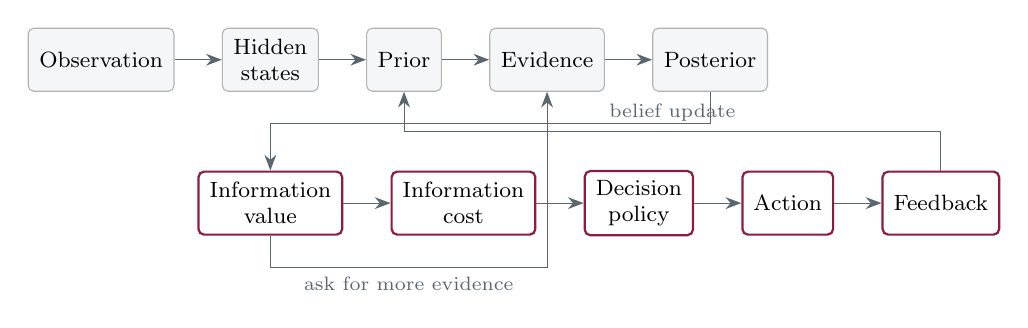
\begin{tikzpicture}[
  node distance=6mm,
  box/.style={draw=sbrule,fill=sbbox,rounded corners=2pt,minimum height=8mm,inner xsep=4pt,font=\footnotesize,align=center},
  new/.style={box,draw=sbaccent,fill=white,thick},
  arr/.style={-{Stealth[length=2mm]},draw=sbsoft}
]
\node[box] (a) {Observation};
\node[box,right=of a] (b) {Hidden\\states};
\node[box,right=of b] (c) {Prior};
\node[box,right=of c] (d) {Evidence};
\node[box,right=of d] (e) {Posterior};

\node[new,below=10mm of b] (f) {Information\\value};
\node[new,right=of f] (g) {Information\\cost};
\node[new,right=of g] (h) {Decision\\policy};
\node[new,right=of h] (i) {Action};
\node[new,right=of i] (j) {Feedback};

\draw[arr] (a)--(b); \draw[arr] (b)--(c); \draw[arr] (c)--(d); \draw[arr] (d)--(e);
\draw[arr] (e.south) -- ++(0,-4mm) -| (f.north);
\draw[arr] (f)--(g); \draw[arr] (g)--(h); \draw[arr] (h)--(i); \draw[arr] (i)--(j);
\draw[arr] (j.north) -- ++(0,5mm) -| node[pos=0.25,above,font=\scriptsize\color{sbsoft}]{belief update} (c.south);
\draw[arr] (f.south) -- ++(0,-4mm) -| node[pos=0.25,below,font=\scriptsize\color{sbsoft}]{ask for more evidence} (d.south);
\end{tikzpicture}
\caption{Week 1 is the top row. Week 2 adds the bottom row and the two loops.
The dark boxes are new.}
\end{figure}

The point is not to make the architecture complicated. The point is that you should be able
to say, for each new box, \emph{why it exists} and \emph{what breaks without it}.

% =====================================================================
\section{Continue the same problem}

Use the same problem you chose in Week 1.

Do not start a new project. Do not choose a new problem. Do not throw away Week 1.

If you genuinely cannot continue your Week 1 problem, say so in your paper and explain why.
That explanation is itself useful research. Do not silently switch.

Throughout this document we use one running example so that every idea has something concrete
attached to it:

\begin{sbrule}
The agent receives an email from a known supplier asking to change the bank account for
future payments. The agent must \textbf{pay}, \textbf{verify}, or \textbf{hold} the request, because the true
identity and intent of the sender are not directly observable.
\end{sbrule}

If your problem is different, the structure still applies. Replace ``supplier'', ``bank change'',
and ``pay'' with your own words. Every table and every calculation in this document has the same
shape for any problem where something important is hidden.

% =====================================================================
\section{Your central research question}
\label{sec:question}

Your whole Week 2 project answers one question:

\begin{sbrule}
How can an AI agent use probabilistic reasoning and information theory to decide
\emph{what it should believe}, \emph{what information it should seek}, and \emph{when it should act}?
\end{sbrule}

You may narrow this question to fit your problem. In fact you should. A narrowed version of
the running example:

\begin{quote}
\itshape
When a supplier requests a bank-account change, which verification step should the agent
perform next, and at what belief should it stop verifying and either pay or hold?
\end{quote}

Write your narrowed question down before you build anything. Put it in the introduction of
your paper. Every section of the paper should visibly serve it.

% =====================================================================
\section{The concepts you need}
\label{sec:concepts}

This section is deliberately not a textbook.

For each concept you get three things: what it means in plain words, a concrete example, and a
\textbf{prompt you can paste into an AI assistant} to learn it properly. You will not find the
equations here. That is on purpose.

Two reasons for that choice. First, a formula you cannot read teaches you nothing, and most of
you are beginners --- reading $-\sum p \log p$ before you understand what it is for is how people
decide they are bad at mathematics. Second, and more importantly, \textbf{going and learning the
thing yourself is the actual assignment.} A brief that hands you every definition trains you to
wait for definitions. Use the prompts. Argue with the answers. Come back with the version you
can explain.

Every concept below carries the same mark:

\vspace{4pt}
\hspace*{0.5em}{\footnotesize\sffamily\color{sbaccent}[extend this yourself]}

\vspace{4pt}
Some of these you have met in a session and some you have not, and it does not matter which. The
instruction is identical either way. Whatever you were given, go past it --- the sessions are a
starting point, never the boundary.

\subsection{How to use the prompts}

Paste the prompt. Read the answer. Then do the part people skip: \textbf{close the chat and write
the explanation in your own words from memory.} If you cannot, you have not learned it. Go back
and ask the assistant to explain it differently.

Every prompt below ends with a line asking the assistant to connect the concept to your problem.
Replace \texttt{[YOUR PROBLEM]} with your own one-sentence problem statement each time. That last
line is what turns a definition into something you can use.

\begin{sbbox}
\boxtitle{Two things the assistant will get wrong}
\textbf{It will over-formalise.} If it answers with notation, reply: ``That was too mathematical.
Explain it again with no symbols at all, using an example a ten-year-old could follow.'' Keep
asking until it lands. This is a normal part of using these tools well.

\textbf{It will agree with you.} If you say ``so entropy is basically accuracy, right?'' it may
well say yes. Test it the other way: ``Give me the strongest reason what I just said is wrong.''
\end{sbbox}

\subsection{The setup we will reuse}

Every example in this document uses one running case, so you can watch the same four hidden
states move through all of the concepts without switching contexts.

\begin{center}
\begin{tabular}{@{}L{4.4cm}C{2.2cm}L{7.4cm}@{}}
\toprule
\textbf{Hidden state} & \textbf{Prior} & \textbf{Meaning} \\
\midrule
Genuine        & 0.40 & The supplier really did change banks. \\
Compromised    & 0.20 & The real supplier's mailbox is under attacker control. \\
Impersonation  & 0.25 & Someone is imitating the supplier from outside. \\
Malicious      & 0.15 & A deliberate fraud attempt, possibly an insider. \\
\bottomrule
\end{tabular}
\end{center}

These four numbers add to 1.00. That is not decoration. It is what makes them a belief. If they
do not add to one, the agent is claiming something is possible that is not on its list, or
claiming the same possibility twice.

\begin{sbbox}
\boxtitle{Where do these four numbers come from?}
Yours will come from one of three places, and you must say which in your paper:
\begin{enumerate}
  \item \textbf{Data.} You counted. ``Of 1{,}200 bank-change requests last year, 480 were genuine.''
  \item \textbf{Domain judgement.} You asked someone who does this job. Say who, and when.
  \item \textbf{Assumption.} You made it up as a starting point. This is allowed. Label it
        clearly as hypothetical.
\end{enumerate}
Inventing numbers and presenting them as measured is the one thing that will fail your
submission. Inventing numbers and labelling them as assumptions is normal research practice.
\end{sbbox}

% ---------------------------------------------------------------
\subsection{Probability and belief \taught}

A probability is a number between 0 and 1 saying how strongly you expect something. It is not a
fact about the world. It is a statement about \emph{your knowledge} of the world.

Two careful people can hold different probabilities for the same event because they have seen
different things. When new evidence arrives both should move, and if they see enough of the same
evidence they should end up close together.

\textbf{Why your agent cares.} An agent that outputs one answer has thrown away everything it
was unsure about. An agent that holds a belief across several possibilities can tell you it is
unsure --- and being able to say ``I don't know'' is what makes escalation to a human possible.

\begin{learnprompt}
I am a beginner. Explain the difference between a probability, a prior, a posterior, and a
likelihood, with no equations at all. Use one everyday example and keep the same example for
all four. Then tell me the most common mistake beginners make in confusing likelihood and
posterior, and give me a test I can use to catch myself making it. Finally connect all four
ideas to this problem: [YOUR PROBLEM].
\end{learnprompt}

% ---------------------------------------------------------------
\subsection{Updating a belief when evidence arrives \taught}

The mechanics are four columns of arithmetic. You should do this by hand at least once, because
seeing it is worth more than being told it.

Say the agent runs an email authentication check (SPF). First it needs to know how often that
check fails \emph{under each hidden state}:

\begin{center}
\begin{tabular}{@{}L{4.4cm}C{3cm}C{3cm}@{}}
\toprule
\textbf{Hidden state} & \textbf{SPF fails} & \textbf{SPF passes} \\
\midrule
Genuine       & 0.02 & 0.98 \\
Compromised   & 0.10 & 0.90 \\
Impersonation & 0.70 & 0.30 \\
Malicious     & 0.60 & 0.40 \\
\bottomrule
\end{tabular}
\end{center}

Read a row as: ``if the message really is from an impersonator, SPF fails 70\% of the time.''
That is a \keyword{likelihood}. It runs in the opposite direction to what you actually want to
know, and getting the direction backwards is the single most common error in this project.

Now suppose SPF fails. Multiply, add, divide:

\begin{center}
\begin{tabular}{@{}L{3.6cm}C{2.4cm}C{2.4cm}C{2.8cm}C{2.4cm}@{}}
\toprule
\textbf{State} & \textbf{Prior} & \textbf{Likelihood} & \textbf{Prior $\times$ Lik.} & \textbf{Posterior} \\
\midrule
Genuine       & 0.40 & 0.02 & 0.008 & 0.027 \\
Compromised   & 0.20 & 0.10 & 0.020 & 0.068 \\
Impersonation & 0.25 & 0.70 & 0.175 & 0.597 \\
Malicious     & 0.15 & 0.60 & 0.090 & 0.307 \\
\midrule
\textbf{Total} & 1.00 & --- & 0.293 & 1.000 \\
\bottomrule
\end{tabular}
\end{center}

Multiply each prior by its likelihood. Add the column. Divide each row by that total. That is
Bayes' theorem, and there is nothing else in it. Belief in impersonation went from 0.25 to 0.60.

\begin{learnprompt}
I am a beginner. Walk me through Bayes' theorem using only a table of numbers and no algebra.
Use a medical test example first, then repeat the identical table structure for this problem:
[YOUR PROBLEM]. Show every arithmetic step. Then tell me what goes wrong if I forget to divide
by the total at the end, and what it means if my likelihoods are the same for every hidden state.
\end{learnprompt}

% ---------------------------------------------------------------
\subsection{Entropy \taught}

Entropy is \textbf{one number that says how confused you are}.

Zero means certain. Higher means your belief is spread out across many possibilities. The unit
is \keyword{bits}, and one bit is roughly ``one good yes/no question's worth of uncertainty''.

\textbf{The example that makes it click.} You are thinking of an animal and I have to guess it.
If there are eight equally likely animals, I need three yes/no questions: halve, halve, halve.
Eight possibilities is three bits. If you tell me it is almost certainly a dog, we are down to
nearly zero bits --- I barely need to ask anything.

For the four hidden states above, entropy is about 1.90 bits. Four equal states would be exactly
2 bits. So the agent's prior is barely better than knowing nothing at all.

\textbf{Why your agent cares.} It converts ``how sure am I?'' into a single number you can track,
compare, and plot. Watching entropy fall as evidence arrives is the clearest picture of your
agent thinking that you will produce all week.

\begin{learnprompt}
I am a beginner and I have never studied information theory. Explain entropy to me with no
formula. Start with the guessing-game intuition, then tell me why the unit is called a bit.
Give me three small examples: a fair coin, a coin that lands heads 99\% of the time, and four
equally likely options. Tell me what entropy is NOT (it is not accuracy, it is not error). Then
show me how to compute it once, by hand, for these four numbers: 0.40, 0.20, 0.25, 0.15 --- and
only then show me the formula, explaining what each piece of it is doing in words. Finally,
connect it to this problem: [YOUR PROBLEM].
\end{learnprompt}

% ---------------------------------------------------------------
\subsection{Information gain \taught}

Information gain is \textbf{how much a question is worth}: how much your confusion drops because
you asked it.

Before the SPF check, the agent sat at 1.90 bits of confusion. If the check comes back
\emph{failed}, the belief becomes the posterior column above and confusion drops to 1.37 bits ---
a drop of 0.53 bits.

\textbf{But here is the part almost everyone gets wrong.} Before you run the check you do not
know whether it will fail. It fails about 29\% of the time and passes about 71\% of the time, and
when it passes it tells you much less (confusion only falls to 1.62 bits). The honest value of
\emph{running} the check is the average across both outcomes, weighted by how likely each outcome
is. That average works out to about \textbf{0.36 bits}, not 0.53.

\begin{sbbox}
\boxtitle{The distinction that decides whether your paper is right}
\textbf{0.53 bits} is what you learned \emph{after} seeing a specific result.

\textbf{0.36 bits} is what the check is worth \emph{before} you run it --- and running it is the
decision you actually have to make.

The second number is called \keyword{expected information gain}. Students routinely compute the
first, call it the second, and rank their evidence sources in the wrong order because of it. If
you take one piece of arithmetic seriously this week, take this one.
\end{sbbox}

\begin{learnprompt}
I am a beginner. Explain information gain with no equations. Use the game of twenty questions.
Then explain the difference between (a) how much I learn after I see a specific answer and
(b) how much I expect to learn before I ask the question, and why (b) is the one I should use to
choose which question to ask. Give me a worked example with small numbers where (a) and (b) are
noticeably different. Then explain why ``is it an animal?'' is often a better question than
``is it a dog?'' even though both are yes/no. Connect it to this problem: [YOUR PROBLEM].
\end{learnprompt}

% ---------------------------------------------------------------
\subsection{Conditional entropy \extend}

Conditional entropy is \textbf{how confused you expect to still be after you get an answer.}

That is the 1.55 bits hiding inside the paragraph above --- the average of 1.37 (if SPF fails)
and 1.62 (if it passes), weighted by how often each happens. Information gain is just the drop
from where you started to there.

\textbf{Why your agent cares.} It is the honest answer to ``how much doubt will remain if I run
this check?'' Some checks leave you in almost exactly the same fog you started in. Conditional
entropy is how you find those before you pay for them.

\begin{learnprompt}
Explain conditional entropy to someone who understands entropy but has never seen the conditional
version, using no formulas. Make clear it is an average over all the answers I might get, not the
entropy after one particular answer. Give me a small worked example with two possible answers
where I can check the arithmetic by hand. Then tell me the relationship between conditional
entropy and information gain in one sentence. Connect it to this problem: [YOUR PROBLEM].
\end{learnprompt}

% ---------------------------------------------------------------
\subsection{Mutual information \extend}

Mutual information asks: \textbf{how much does knowing one thing tell me about another thing?}

If it is zero, the two are unrelated and one is useless for predicting the other. The higher it
is, the more one reveals about the other.

Here is the small surprise worth putting in your paper: \textbf{mutual information and expected
information gain are the same quantity}. Two communities named the same idea differently ---
decision trees say ``information gain'', communication theory says ``mutual information''. When
you notice that two things you learned separately are one thing, you have understood both.

\begin{sbbox}
\boxtitle{Mutual information catches what correlation misses}
Take a number that can be $-2$, $-1$, $1$, or $2$, each equally likely. Now square it, giving 4,
1, 1, or 4.

\textbf{Correlation between the two is exactly zero.} The relationship is perfectly symmetric so
it cancels itself out, and any correlation-based tool will report ``no relationship here''.

\textbf{But knowing the first number tells you the second one perfectly.} Mutual information is
1 bit --- the maximum possible.

Correlation asks ``do these move together in a straight line?'' Mutual information asks ``does
knowing one reduce my uncertainty about the other \emph{in any way at all}?'' For agent design
the second question is the one you want, because your most useful evidence is very often not
linearly related to your hidden state.
\end{sbbox}

\begin{learnprompt}
Explain mutual information to a beginner with no formulas. Tell me intuitively what it measures
and what it means when it is zero. Then explain how it differs from correlation, using the
example of a number and its square, and give me one more example from everyday life where two
things are strongly related but correlation would report nothing. Then tell me why mutual
information is symmetric and what that symmetry means practically. Finally, tell me how I could
use it to decide whether an evidence source is worth collecting for this problem: [YOUR PROBLEM].
\end{learnprompt}

% ---------------------------------------------------------------
\subsection{Cross-entropy \extend}

Cross-entropy is \textbf{a score for how surprised your model is by reality}, on average. Lower
is better. It is lowest when your model's beliefs match what actually happens.

\textbf{The property that matters.} It punishes being \emph{confidently wrong} far more harshly
than being unsure. Suppose the truth turns out to be A. If your model gave A a 50\% chance, it
pays a small penalty. If your model gave A a 1\% chance, it pays a penalty roughly seven times
larger. Confidence is only cheap when you are right.

This is why almost every classifier you will ever train is trained on cross-entropy, and it is
also the behaviour you want in your agent: an agent that says ``99\% safe'' about a fraudulent
payment should be penalised much harder than one that shrugged and said ``50/50''.

\begin{learnprompt}
Explain cross-entropy to a beginner with no equations. Frame it as ``how surprised is my model,
on average, by what really happens''. Show me with three small examples why being confidently
wrong is punished much harder than being uncertain. Then explain why this is the loss function
used to train classifiers, and what would go wrong if we used plain accuracy instead. Connect it
to why a confident, badly calibrated AI agent is dangerous in this problem: [YOUR PROBLEM].
\end{learnprompt}

% ---------------------------------------------------------------
\subsection{KL divergence \extend}

KL divergence measures \textbf{how far apart two beliefs are} --- specifically, how much you lose
by believing the wrong one. It is zero when the two are identical.

You will hear it called a ``distance''. It is not one, and the reason is worth understanding.

\begin{sbbox}
\boxtitle{The example that shows why it is not a distance}
Reality: a fair coin. Heads half the time, tails half the time.

Your model: ``heads, always. Tails is impossible.''

\textbf{Measured one way}, the disagreement is \emph{infinite}. Half the time reality produces
tails --- an event your model called impossible --- and being surprised by an impossible event is
infinitely costly.

\textbf{Measured the other way round}, the disagreement is small and finite.

Same two beliefs, two different answers depending on which one you put first. A real distance
cannot do that; the distance from Delhi to Mumbai does not depend on which city you name first.
So KL divergence is called a \emph{divergence}.

\textbf{The lesson for your agent, and it is a serious one:} assigning zero probability to
something that can actually happen is the most dangerous modelling error available to you. If
``insider fraud'' is not on your hidden-state list, no amount of evidence will ever make your
agent consider insider fraud. It is not unlikely in your model. It is \emph{impossible} in your
model, and your agent will be infinitely surprised on the day it happens.

This is why Section~\ref{sec:probview} tells you to include a residual ``something else'' state.
\end{sbbox}

\begin{learnprompt}
Explain KL divergence to a beginner with no formulas. Start with what it is for: comparing two
probability distributions, one of which is usually reality and one of which is usually my model.
Explain what it means when it is zero. Then explain clearly why it is asymmetric, and construct
a simple two-outcome example where measuring it one way gives a much bigger number than the other
way. Explain why assigning zero probability to a possible event makes it infinite, and why that
is a warning to anyone designing an AI agent. Only after all of that, show me the formula and
explain what each piece is doing. Connect it to this problem: [YOUR PROBLEM].
\end{learnprompt}

% ---------------------------------------------------------------
\subsection{Jensen--Shannon divergence \extend}

Once you know KL divergence is asymmetric and can blow up to infinity, the obvious next question
is: \emph{is there a fixed version?} There is. That question --- and following it --- is exactly
the behaviour this course is trying to build in you.

Jensen--Shannon divergence compares two beliefs by measuring each one against their average
instead of against each other. Three things follow, and all three are practical:

\begin{itemize}
  \item \textbf{It is symmetric.} Order does not matter any more.
  \item \textbf{It never goes to infinity}, even when one belief says something is impossible.
  \item \textbf{It is bounded}, so the number means something on its own rather than only in
        comparison.
\end{itemize}

\textbf{Why your agent cares, concretely.} Take the pattern of evidence your agent saw last
quarter and the pattern it is seeing this month. Compare them. If the number jumps, the world has
moved and your priors are now describing a world that no longer exists. That is a
\keyword{distribution shift} alarm, built out of one idea from information theory --- and KL
divergence would have been the natural first choice and would have returned infinity the first
time a genuinely new kind of evidence showed up.

\begin{learnprompt}
I understand that KL divergence is asymmetric and can be infinite. Explain Jensen--Shannon
divergence to me as the fix for those two problems, with no formulas at first. Explain the idea
of comparing both distributions to their average and why that repairs both problems. Tell me what
it means that it is bounded, and what its square root gives me. Then give me a practical example
of using it to detect that the world has changed since a model was built. Finally show me the
formula and explain each piece. Connect it to this problem: [YOUR PROBLEM].
\end{learnprompt}

% ---------------------------------------------------------------
\subsection{Calibration \extend}

An agent is \keyword{calibrated} if, across all the cases where it said ``80\% likely'', the
thing actually happened about 80\% of the time.

\textbf{This is not the same as accuracy}, and the difference matters enormously. An agent can be
95\% accurate and badly calibrated: it says ``99\% certain'' about everything, is right 95\% of
the time, and is therefore overconfident on every single case it ever sees.

\begin{sbbox}
\boxtitle{Why a confident agent can be more dangerous than an uncertain one}
An uncertain agent escalates to a human. Its uncertainty is a signal that switches on a safety
mechanism.

An overconfident agent never escalates. It is wrong at exactly the same rate --- it has simply
removed the one control that would have caught its mistakes.

Confidence is not a virtue in an agent. Calibrated confidence is. And every downstream thing you
build this week --- your threshold, your expected-cost calculation, your stop rule --- takes the
agent's probabilities at face value. If those numbers are dishonest, everything built on them is
dishonest too.
\end{sbbox}

\textbf{How to check it.} Bucket your agent's predictions (0--10\%, 10--20\%, and so on). For each
bucket, compare the average confidence it stated against how often it was actually right. A
calibrated agent's points sit on the diagonal. This plot has a name and there is a standard
summary number for the gap --- find both.

\begin{learnprompt}
Explain calibration for a beginner, with no formulas. Make the difference between accuracy and
calibration very clear with an example of a model that is highly accurate and badly calibrated,
and another that is less accurate but well calibrated. Tell me which one I would rather deploy in
a system that escalates uncertain cases to a human, and why. Then tell me the name of the standard
plot for checking calibration and the standard number that summarises the error, and explain how
to build both from a table of predictions and outcomes. Explain why large language models are
often poorly calibrated. Connect this to this problem: [YOUR PROBLEM].
\end{learnprompt}

% ---------------------------------------------------------------
\subsection{Expected value and expected cost \taught}

Expected value is what you get on average if you make the same choice many times: each outcome
weighted by how likely it is. Expected cost is the same idea, counting losses instead.

The rule your agent lives by follows from this, and it is not obvious:

\begin{sbrule}
The agent should \textbf{not} choose the most likely state.
The agent should choose the \textbf{action with the lowest expected cost}.
\end{sbrule}

Those are frequently different actions. If a fraudulent payment costs four hundred times more
than annoying a supplier, the agent should hold the payment even when it is fairly confident the
request is genuine. ``Most likely'' and ``best'' are simply not the same question, and
Section~\ref{sec:decision} works out exactly where they part company.

\begin{learnprompt}
Explain expected value and expected cost to a beginner with no formulas, using a bet and then an
insurance decision. Then explain, with a concrete example, why the action with the highest
probability of being right is sometimes not the action you should take. Make the example one
where the two errors have very different costs. Finally explain what ``opportunity cost'' means
in that same example. Connect it to this problem: [YOUR PROBLEM].
\end{learnprompt}

% ---------------------------------------------------------------
\subsection{Value of information \extend}

This is the most important idea in Week 2, so read this subsection twice.

Value of information is \textbf{how much better off you are for having asked}, minus what asking
cost you.

Notice what it is \emph{not} measured in. It is not measured in bits. It is measured in whatever
your outcomes are measured in --- rupees, hours, lives, reputation, delay.

\begin{sbrule}
Information has value only when some possible answer would make you \textbf{do something
different}.

If every answer leads to the same action, the value of that information is zero, minus its cost.
Do not buy it --- no matter how many bits it carries.
\end{sbrule}

That rule is the whole of Section~\ref{sec:challenge}, and it is where most students' thinking
changes this week.

\begin{learnprompt}
Explain ``value of information'' to a beginner with no formulas. Make the key point very clearly:
information is only worth something if it could change what I decide to do. Give me one example
where an extremely informative test is worthless because it cannot change the decision, and one
example where a cheap, much less informative test is worth buying. Then explain how to decide
whether to pay for a test, in plain steps I can follow. Explain when I should stop gathering
information entirely. Connect it to this problem: [YOUR PROBLEM].
\end{learnprompt}

% ---------------------------------------------------------------
\subsection{Exploration and exploitation \extend}

\keyword{Exploitation} is acting on what you already believe. \keyword{Exploration} is paying
something now to learn something that improves your later decisions.

Your agent faces this every time it considers a verification step. Skipping the phone call is
exploitation. Making the call is exploration. A pure exploiter is fast and eventually wrong in a
way it never finds out about. A pure explorer never gets anything done.

Your stop rule, in Section~\ref{sec:decision}, is your answer to this trade-off. Present it as
one.

\begin{learnprompt}
Explain exploration versus exploitation to a beginner with no formulas or algorithms. Use an
everyday example like choosing a restaurant. Then explain what goes wrong at each extreme: an
agent that only exploits, and an agent that only explores. Tell me the common simple strategies
people use to balance the two and what each one assumes. Connect it to an agent that must decide
whether to run one more verification check before acting on this problem: [YOUR PROBLEM].
\end{learnprompt}

% ---------------------------------------------------------------
\subsection{Distribution shift \extend}

Your agent's priors were set from how the world used to be. Distribution shift is what happens
when the world stops being that way and nobody tells the agent.

The dangerous part is that nothing breaks loudly. The agent keeps producing confident answers
from beliefs that no longer describe anything real. Fraud tactics change. A supplier gets
acquired. Your company enters a new market. Your priors quietly become fiction.

\textbf{Why your agent cares.} Detecting this is one of the few genuinely open problems you can
touch this week. The Jensen--Shannon alarm described above is one workable answer. There are
others. Finding a second one and comparing them would make an excellent contribution.

\begin{learnprompt}
Explain distribution shift to a beginner with no formulas. Distinguish clearly between the input
data changing and the underlying relationship changing, and give an example of each. Then explain
why a model can keep producing confident answers while being completely wrong, and why nobody
notices for a long time. Give me three practical ways a deployed system could detect that it has
happened, and the weakness of each. Finally, tell me what a system should actually do once it
suspects the world has shifted. Connect it to this problem: [YOUR PROBLEM].
\end{learnprompt}

% ---------------------------------------------------------------
\subsection{The whole set, on one page}

\begin{center}
\small
\begin{tabular}{@{}L{4.2cm}L{10.4cm}@{}}
\toprule
\textbf{Concept} & \textbf{Why your agent needs it} \\
\midrule
Probability, belief   & Lets the agent hold several explanations instead of guessing one. \\
Belief update (Bayes) & Turns evidence into a changed mind. \\
Entropy               & One number for how confused the agent is right now. \\
Information gain      & How much a question is worth before you ask it. \\
Conditional entropy   & How much doubt will still remain after you ask. \\
Mutual information    & Whether an evidence source is related to what you care about at all. \\
Cross-entropy         & Scores a model, and punishes confident wrongness hardest. \\
KL divergence         & Compares two beliefs; warns you about impossible-in-model events. \\
Jensen--Shannon divergence & The symmetric, finite version; a practical drift alarm. \\
Calibration           & Whether the agent's confidence can be trusted at all. \\
Value of information  & Whether an answer is worth what it costs. \\
Exploration and exploitation & When to stop asking and act. \\
Distribution shift    & Whether the agent's priors still describe the real world. \\
\bottomrule
\end{tabular}
\end{center}

Thirteen concepts, one instruction for all of them: go further than you were given.

\begin{sbbox}
\boxtitle{These prompts teach you concepts. They do not do your project.}
Everything above is a prompt to \emph{understand something}. None of them asks an assistant to
produce your hidden states, your priors, your costs, your results, or your paragraphs.

Keep that line where it is. A concept explained to you is yours once you can re-explain it. A
result generated for you is never yours, and you will not survive the first question about it.
\end{sbbox}


\section{The extension rule}
\label{sec:nottaught}

Your paper must contain concepts you went and found for yourself. Sessions and briefs are a
starting point. Neither is a syllabus, and neither is a boundary.

We are not testing whether you can memorise a syllabus. We are testing whether, when you hit
the edge of what you were told, you can push one step further on your own. This is the single
most transferable skill in this course.

The behaviour looks like this. You take something you know, ask the obvious next question, and
follow it:

\begin{center}
\begin{tabular}{@{}L{7.6cm}L{7.2cm}@{}}
\toprule
\textbf{You were taught} & \textbf{The question that takes you further} \\
\midrule
Entropy measures uncertainty. & ``What if I want to compare two beliefs, not measure one?'' $\rightarrow$ KL divergence \\
KL divergence compares distributions. & ``It gives different answers depending on the order. Is there a symmetric version?'' $\rightarrow$ Jensen--Shannon divergence \\
Information gain tells me a question's value. & ``How much does observing $X$ tell me about $Y$ specifically?'' $\rightarrow$ Mutual information \\
Mutual information measures dependence. & ``How is that different from correlation?'' $\rightarrow$ Non-linear dependence \\
The agent outputs a probability. & ``Is that number trustworthy?'' $\rightarrow$ Calibration, reliability diagrams \\
The agent has priors. & ``What if the world changed since I set them?'' $\rightarrow$ Distribution shift \\
The agent picks the best question. & ``What if the best question is expensive?'' $\rightarrow$ Value of information \\
\bottomrule
\end{tabular}
\end{center}

Section~\ref{sec:concepts} walks the first few steps of this ladder with you and gives you
thirteen concepts to extend. Those thirteen are the floor, not the ceiling.

\textbf{Do not stop where this document stops.} Find at least two concepts that are not in this
document at all. Learn them well enough to explain simply. Use them for something real. Name
them in your paper and say how you found them.

\begin{sbbox}
\boxtitle{Where the next two concepts come from}
Not from a list. From your own results.

The move is always the same: something in your project does not work, or works for a reason you
cannot explain, and you go looking for the name of it. ``My agent is 94\% accurate and still
loses money'' sends you towards cost-sensitive learning. ``My two evidence sources keep agreeing
even when they are both wrong'' sends you towards conditional independence. ``I have almost no
fraud cases in my data'' sends you towards class imbalance.

A student who collects concepts from a syllabus produces a paper that lists them. A student who
collects concepts from their own failures produces a paper that uses them. We can tell the
difference immediately, and so can an interviewer.

The general-purpose prompt, when you have a name but no understanding:

\begin{quote}\ttfamily\small\raggedright
Explain [CONCEPT] to me as if I have never studied machine learning.
Give me the plain-English meaning first, in three sentences and no symbols.
Then give me one worked example with numbers small enough for me to check by hand.
Then tell me one situation where using this concept would be a mistake.
Then connect it to this problem: [YOUR PROBLEM].
\end{quote}

The last two lines matter most. A concept you cannot misuse is a concept you have not
understood, and a concept you cannot connect to your problem does not belong in your paper.

Then close the chat and write the explanation in your own words from memory. If you cannot, you
have not learned it yet. Go back.
\end{sbbox}

% =====================================================================
\section{Reading papers (optional this week)}
\label{sec:reading}

There is no mandatory reading list for Week 2.

If you want to read research papers, do. Choose beginner-friendly ones connected to your own
problem. Good starting points are survey articles, blog explanations by the authors, and the
introduction sections of papers --- which are usually written for outsiders even when the rest
is not.

If you do read something, do not summarise it in your paper. Connect it. For each paper or
article, answer these, briefly:

\begin{enumerate}[itemsep=1pt]
  \item What problem is it solving?
  \item What is the simplest version of the idea?
  \item What does it assume?
  \item What information does the system use, and what decision does it make?
  \item What is the main experiment, and what did the authors find?
  \item What limitation did you notice?
  \item \textbf{How does this change my agent's design?}
\end{enumerate}

The last one is not optional. If a paper changed nothing in your design, it does not belong in
your Related Work section.

\begin{sbbox}
\boxtitle{Two rules that do not bend}
\textbf{Never cite something you did not read.} An AI assistant can produce a plausible citation
list in two seconds. Some of those papers will not exist. Every reference in your bibliography
must be something you opened.

\textbf{Never publish a claim you cannot explain.} If someone asks you at an interview what your
paper meant on page 4 and you cannot answer, the paper is not yours.

It is perfectly fine to use an AI assistant to make a hard paper readable. Ask it to explain the
paper in simple language, then verify the explanation against the actual paper. That is
research. Pasting its summary into your Related Work section is not.
\end{sbbox}

\textbf{Optional exercise, strongly recommended.} Take one paper or article and prepare a
five-minute explanation for a friend who has never studied machine learning. Cover: the problem,
the intuition, what the researchers actually did, what happened, what it fails to explain, and
how it connects to your agent. If you can do this without looking at the PDF, you understand it.

% =====================================================================
\section{Build the probabilistic view of your agent}
\label{sec:probview}

Rebuild your Week 1 architecture with these twelve components. For each one, write a short
paragraph about \emph{your} problem. This becomes Section 5 of your paper.

\begin{center}
\begin{longtable}{@{}C{0.8cm}L{3.5cm}L{9.9cm}@{}}
\toprule
\textbf{\#} & \textbf{Component} & \textbf{The question it answers} \\
\midrule
\endhead
1  & Observation      & What does the agent actually receive? Be concrete. Not ``an email'' but ``sender address, display name, SPF/DKIM result, message body, attachment, thread history''. \\
2  & Hidden state     & What is genuinely unknown and matters? Usually: who this really is, or what they intend. \\
3  & Possible worlds  & What are all the plausible explanations? List every one, including boring ones. Include a residual ``something else'' state. \\
4  & Prior belief     & What did the agent believe before this evidence? Where did that number come from? \\
5  & Evidence         & What new signals can arrive or be requested? \\
6  & Posterior belief & How does belief change? Show one full Bayes calculation by hand in the paper. \\
7  & Uncertainty      & How confused is the agent now? Report entropy in bits. \\
8  & Information value& Which available evidence would reduce that uncertainty most? \\
9  & Cost             & What does obtaining it cost in money, time, human attention, and relationship damage? \\
10 & Decision         & Which action minimises expected cost, given the belief and the costs? \\
11 & Feedback         & What happens after acting, and when do you find out you were wrong? \\
12 & Belief update    & How does the outcome change future priors? \\
\bottomrule
\end{longtable}
\end{center}

\begin{sbbox}
\boxtitle{Component 11 is the one people skip}
Feedback delay decides how much your agent can learn. If a wrong ``pay'' decision is discovered
in two days, you can update quickly. If it surfaces at the quarterly audit, your agent runs
blind for three months and its priors slowly drift away from reality.

Worse, feedback is usually \emph{asymmetric}. When the agent holds a payment, someone complains
and you learn immediately that it was genuine. When the agent pays a fraudster, nobody complains.
So the agent hears about its false positives loudly and its false negatives never. An agent that
learns from this feedback will drift towards paying everything. Write about this. It is real, it
affects almost every problem in this cohort, and it is exactly the kind of observation that makes
a paper good.
\end{sbbox}

% =====================================================================
\section{The belief-state table}
\label{sec:belieftable}

Build this table for your own problem. It is the spine of your paper.

\begin{center}
\begin{tabular}{@{}L{3.1cm}C{1.6cm}L{4.1cm}C{1.8cm}L{2.6cm}@{}}
\toprule
\textbf{Hidden state} & \textbf{Prior} & \textbf{Evidence observed} & \textbf{Posterior} & \textbf{Implied action} \\
\midrule
Genuine       & 0.40 & SPF fail, new account & 0.03 & Hold \\
Compromised   & 0.20 & SPF fail, new account & 0.07 & Verify \\
Impersonation & 0.25 & SPF fail, new account & 0.60 & Hold \\
Malicious     & 0.15 & SPF fail, new account & 0.30 & Hold \\
\midrule
\multicolumn{2}{@{}l}{Entropy} & 1.90 bits $\rightarrow$ & 1.37 bits & \\
\bottomrule
\end{tabular}
\end{center}

\emph{These numbers are illustrative and hypothetical. Yours must be your own.}

Rules for this table:

\begin{itemize}
  \item Priors must sum to 1.00. Posteriors must sum to 1.00. Check the arithmetic.
  \item State where each prior came from --- data, judgement, or assumption.
  \item Show at least one posterior worked out in full, the way Section~\ref{sec:concepts} does.
        Not the final number only.
  \item Report entropy before and after. It makes the update visible as one number.
  \item If the numbers are hypothetical, write the word ``hypothetical'' next to them.
\end{itemize}

\begin{sbbox}
\boxtitle{On honesty with numbers}
Hypothetical numbers, clearly labelled, are completely acceptable and normal at this stage.

Hypothetical numbers presented as measured results are academic fraud. There is no middle
ground and no partial credit. If you did not run it, do not report it.
\end{sbbox}

% =====================================================================
\section{Information selection: which evidence next?}
\label{sec:infoselect}

Your agent has several things it could check. It cannot check everything, and it should not.

Compare at least \textbf{three} evidence sources. For each one, answer all eight questions below.
Here is a fully worked comparison from the running example, using the priors from
Section~\ref{sec:concepts}.

\subsection{Three candidate checks}

\textbf{Check A --- SPF/DKIM authentication result.} Already computed:
expected information gain $= 0.36$ bits. Cost: effectively zero. Time: milliseconds.

\textbf{Check B --- Has this supplier used this bank account before?} A lookup in the payments
database.

\begin{center}
\begin{tabular}{@{}L{4.0cm}C{3.2cm}C{3.4cm}@{}}
\toprule
\textbf{Hidden state} & $P(\text{new account}\mid S)$ & $P(\text{known account}\mid S)$ \\
\midrule
Genuine       & 0.30 & 0.70 \\
Compromised   & 0.90 & 0.10 \\
Impersonation & 0.95 & 0.05 \\
Malicious     & 0.95 & 0.05 \\
\bottomrule
\end{tabular}
\end{center}

The account comes back \emph{new} 68\% of the time, leaving the belief at
$(0.177,\, 0.265,\, 0.349,\, 0.210)$ and confusion at 1.95 bits. It comes back \emph{known} 32\%
of the time, leaving $(0.875,\, 0.063,\, 0.039,\, 0.023)$ and confusion at 0.73 bits.

Average those two, weighted by how often each happens: $0.68 \times 1.95$ plus
$0.32 \times 0.73$ is 1.56 bits of remaining confusion. Starting from 1.90, this check is worth
\textbf{0.34 bits}.

\textbf{Check C --- Phone the supplier on the number already on file} (not any number in the
email) and ask them to confirm.

\begin{center}
\begin{tabular}{@{}L{4.0cm}C{3.2cm}C{3.4cm}@{}}
\toprule
\textbf{Hidden state} & \textbf{Supplier confirms} & \textbf{Does not confirm} \\
\midrule
Genuine       & 0.95 & 0.05 \\
Compromised   & 0.30 & 0.70 \\
Impersonation & 0.05 & 0.95 \\
Malicious     & 0.05 & 0.95 \\
\bottomrule
\end{tabular}
\end{center}

The supplier confirms 46\% of the time, leaving 0.85 bits of confusion. They do not confirm 54\%
of the time, leaving 1.71 bits.

Averaged the same way, 1.31 bits of confusion remain. Starting from 1.90, this check is worth
\textbf{0.59 bits} --- the most informative of the three.

\subsection{The comparison table}

\begin{center}
\small
\begin{tabular}{@{}L{2.6cm}C{1.5cm}C{1.5cm}C{1.6cm}C{1.9cm}L{4.0cm}@{}}
\toprule
\textbf{Evidence} & \textbf{Exp.\ IG} & \textbf{Cost} & \textbf{Time} & \textbf{Bits per \rs 100} & \textbf{If it is wrong} \\
\midrule
A. SPF/DKIM & 0.36 bits & $\approx$\rs 0 & 200\,ms & very large & Forwarding and mailing lists break SPF. Genuine mail fails. \\[3pt]
B. Bank-account history & 0.34 bits & $\approx$\rs 2 & 2\,s & 17.0 & Supplier really did switch banks. Legitimate change looks new. \\[3pt]
C. Phone callback & 0.59 bits & \rs 300 & 30\,min & 0.20 & Wrong number on file, or the person who answers was also deceived. \\[3pt]
D. Full forensic audit & 0.90 bits & \rs 10{,}000 & 2\,days & 0.009 & Rarely wrong, but the request is stale by the time it finishes. \\
\bottomrule
\end{tabular}
\end{center}

\emph{Illustrative numbers. Cost for A and B is amortised infrastructure cost; cost for C is
30 minutes of analyst time.}

\subsection{What this table already tells you}

Three things worth writing about in your paper, all visible in the numbers above.

\textbf{First, the most informative check is the worst value.} The forensic audit carries the
most bits and is close to useless in practice: 0.009 bits per hundred rupees, against 17 bits
for the database lookup. Ranking evidence by information alone gives you exactly the wrong order.

\textbf{Second, cheap checks should run first, always.} A and B together cost about two rupees and
two seconds. There is no situation where you would skip them. Order matters: run the free checks,
then re-evaluate whether the expensive one is still needed. Often it is not, because the belief
has already crossed a threshold.

\textbf{Third, and most interesting: information can increase uncertainty.} Look at Check B. Prior
entropy is 1.90 bits. If the account comes back \emph{new}, posterior entropy is \textbf{1.95 bits}.
The agent knows more and is more confused than before.

This is not a bug and it is not an error in the arithmetic. Before the check, the agent leaned
towards ``genuine'' at 0.40. Finding a new account knocks ``genuine'' down and leaves three
remaining explanations at roughly similar strength --- and a flat belief has high entropy. The
agent has correctly moved from ``probably fine'' to ``definitely something, but I do not know
which something''.

\begin{sbbox}
\boxtitle{Reconciling this with the theory}
\emph{Expected} information gain is never negative: $I(S;E) \geq 0$ always. On average, evidence
helps. But the gain from any \emph{single outcome} can absolutely be negative. Averaged over both
outcomes, Check B still gives $+0.34$ bits.

This is a direct, worked answer to Advanced Question~4, taken from a real design rather than a
textbook. If you find something like this in your own problem, that is exactly the kind of
finding to build a LinkedIn post around.
\end{sbbox}

% =====================================================================
\section{Design five questions your agent could ask}
\label{sec:questions}

Write five. Fill this table. Then explain which one the agent actually picks and why.

\begin{center}
\small
\begin{tabular}{@{}L{3.6cm}L{2.4cm}C{1.3cm}C{1.2cm}C{1.2cm}L{2.8cm}@{}}
\toprule
\textbf{Question} & \textbf{Possible answers} & \textbf{Info value} & \textbf{Cost} & \textbf{Time} & \textbf{Would ask?} \\
\midrule
Has this supplier used this account before? & new / known & 0.34 bits & \rs 2 & 2\,s & Yes, always \\[3pt]
Did the message pass SPF and DKIM? & pass / fail / none & 0.36 bits & \rs 0 & 200\,ms & Yes, always \\[3pt]
Does the request match this supplier's historical pattern? & typical / unusual & 0.21 bits & \rs 5 & 5\,s & Yes, always \\[3pt]
Can the supplier confirm on the number already on file? & confirms / denies / unreachable & 0.59 bits & \rs 300 & 30\,min & Only if still uncertain after the cheap checks \\[3pt]
Was the request sent from a device or IP seen before? & known / new & 0.28 bits & \rs 40 & 3\,min & Only if callback fails or is unreachable \\
\bottomrule
\end{tabular}
\end{center}

\emph{Illustrative numbers.}

Now write the reasoning explicitly. For the table above it reads:

\begin{quote}\itshape
The agent always runs the three cheap checks first, in any order, because they cost under ten
rupees combined and complete in seconds. It then recomputes its belief. If the posterior
probability of a bad state is below 0.5\% or above 60\%, it acts immediately --- the callback
cannot change the decision, so its value of information is zero regardless of its bit count. It
places the callback only in the middle band, where the extra 0.59 bits can actually flip the
action. The device check is a fallback for when the supplier cannot be reached.
\end{quote}

Notice the structure of that paragraph: cheap first, recompute, then ask whether the expensive
check could \emph{change the decision}, and only spend if it could. That is the whole policy in
four sentences. Yours should be similarly explicit.

% =====================================================================
\section{Critical thinking challenge}
\label{sec:challenge}

\begin{sbrule}
\textbf{Is the question that gives the most information always the best question?}
\end{sbrule}

This section is mandatory. Do not answer with a definition. Answer with numbers from your own
problem.

Here is what a complete answer looks like, using the running example.

\subsection{The naive answer}

Rank by information gain: the forensic audit wins with 0.90 bits, the callback is second with
0.59. Always run the audit.

\subsection{Why that is wrong}

Bits are not the objective. Money, time, and correct decisions are the objective. Bits are only
useful when they change what you do.

Take a request where the cheap checks have already left the agent at $P(\text{bad}) = 0.75$. The
threshold for holding (derived in Section~\ref{sec:decision}) is $0.0025$. The agent is far
above it. It will hold this payment.

Now ask the decisive question: \emph{is there any outcome of the forensic audit that changes that
action?} If the audit comes back clean, the posterior drops --- but not below 0.0025. The agent
still holds. If it comes back dirty, the agent holds.

The audit carries 0.90 bits and changes nothing. It saves \rs 0 and costs \rs 10{,}000, so its
value of information is minus ten thousand rupees. The most informative question available is
the worst thing the agent could do.

\subsection{The rule that follows}

\begin{sbbox}
\boxtitle{Information only has value when it can change an action}
Before paying for any evidence, ask: \emph{is there an outcome of this check that would make me do
something different?}

If no, the value of that information is zero, minus its cost. Do not buy it. This holds no matter
how many bits it carries.

If yes, compare the expected cost saved against the cost of obtaining it. Buy it only if the
saving is larger.
\end{sbbox}

\subsection{The case where it does pay}

Take a request sitting at $P(\text{bad}) = 0.35$, on a payment of \rs 8{,}00{,}000.

\begin{itemize}
  \item Hold now: the request is genuine with probability 0.65, so expected cost of a wrong hold
        is $0.65 \times \rs 2{,}000 = \rs 1{,}300$.
  \item Pay now: expected cost is $0.35 \times \rs 8{,}00{,}000 = \rs 2{,}80{,}000$.
  \item Callback for \rs 300: it resolves most of the ambiguity. If the supplier confirms, the
        agent pays with far more confidence. If not, it holds with far more confidence. The
        expected cost after the callback drops to roughly \rs 900.
\end{itemize}

Value of information $\approx \rs 1{,}300 - \rs 900 - \rs 300 = \rs 100$. Positive, so make the
call. Marginally --- and that is realistic. Most good decisions are not dramatic.

\subsection{What to write in your paper}

Give one case from your problem where the highest-information question is the right choice, and
one case where it is not. Show the numbers. State the rule you extracted. Two paragraphs is
enough if the numbers are real.

% =====================================================================
\section{Decision-making under uncertainty}
\label{sec:decision}

Your agent does not need certainty. It needs a rule for when it has enough.

\subsection{Where thresholds actually come from}

Most students write ``if the probability of fraud exceeds 80\%, hold the request.'' Then the
obvious question: \textbf{why 80\%?} Why not 70\%, or 90\%?

The honest answer is that 80\% came from nowhere. Thresholds are not chosen. They are
\emph{derived} from the cost of being wrong in each direction.

Two errors, two costs:

\begin{itemize}
  \item \textbf{False positive}: hold a genuine request. It costs \rs 2{,}000 --- delay, supplier
        annoyance, some staff time.
  \item \textbf{False negative}: pay a fraudulent request. It costs \rs 8{,}00{,}000 --- the
        payment, mostly unrecoverable.
\end{itemize}

Now find the belief at which the two mistakes cost the same. Below it you should pay; above it
you should hold. There is one line of arithmetic, and you can do it in your head:

\begin{sbrule}
\textbf{Break-even belief} \;=\; cost of a false positive \;$\div$\; (cost of a false positive
$+$ cost of a false negative)

\vspace{3pt}
$2{,}000 \div (2{,}000 + 8{,}00{,}000) \;=\; \mathbf{0.0025}$, or one quarter of one percent.
\end{sbrule}

\begin{sbbox}
\boxtitle{The threshold is 0.25\%, not 80\%}
This result surprises almost everyone the first time. It follows directly from the costs. Paying
a fraud is 400 times more expensive than annoying a supplier, so the agent should hold on a
quarter of a percent of suspicion.

Answer the follow-up before your reader asks it: \emph{if the threshold is really 0.25\%, does the
agent hold everything?} Nearly, if ``pay'' and ``hold'' are the only two actions. Which is why
real systems have a third action.

The verify action costs \rs 300 and resolves most of the doubt. With three actions the policy
becomes: pay below $p_{\text{low}}$, verify between $p_{\text{low}}$ and $p_{\text{high}}$, hold
above $p_{\text{high}}$. The cheap middle action is what makes the system usable. This is the
central design insight of the whole exercise, and it falls out of the arithmetic rather than out
of intuition.
\end{sbbox}

\subsection{What you must answer about your threshold}

\begin{enumerate}
  \item What is your threshold, and what cost ratio produced it?
  \item What happens at a threshold ten points lower? How many more false positives?
  \item What happens ten points higher? How many more false negatives?
  \item What is the cost of a false positive in your problem? Include the non-monetary parts.
  \item What is the cost of a false negative? Same.
  \item Should the threshold move with context --- payment size, supplier age, time of month?
  \item Which cases go to a human regardless of the probability?
\end{enumerate}

Question 6 deserves real thought. A single fixed threshold implicitly claims that a
\rs 5{,}000 payment and a \rs 50{,}00{,}000 payment deserve identical scrutiny. They do not,
and your own arithmetic already knows this: the cost of a false negative grows with the payment,
so the break-even belief should fall as the amount rises. A threshold that moves with the stakes is a stronger design than a constant,
and it costs you one line of code.

\subsection{The stop rule}

When should the agent stop gathering and act? Any of these, whichever comes first:

\begin{enumerate}
  \item \textbf{No remaining check can change the action.} Value of information is zero. Act.
  \item \textbf{The best remaining check costs more than it saves.} Negative value of information. Act.
  \item \textbf{Belief is outside the uncertain band.} Above $p_{\text{high}}$ or below $p_{\text{low}}$. Act.
  \item \textbf{Time ran out.} Some decisions expire. Act on the default safe action.
  \item \textbf{Evidence stopped moving the belief.} Two checks in a row changed the posterior by
        less than some small amount. Further checks are probably measuring the same thing twice.
\end{enumerate}

Rule 5 is worth investigating. Correlated evidence sources feel like more information and are
not. Three sources that all key on the same underlying signal give you roughly one source's
worth of bits while charging you three times.

\subsection{Human escalation}

Say explicitly when a human is involved. Reasonable triggers:

\begin{itemize}
  \item The belief sits in the uncertain band after all affordable checks are exhausted.
  \item The cost of a wrong decision exceeds some ceiling, regardless of confidence.
  \item Two evidence sources disagree strongly.
  \item The case looks unlike anything in the historical data --- a possible new hidden state.
  \item The agent's calibration has been drifting recently.
\end{itemize}

Note that the second trigger has nothing to do with probability. Some decisions should reach a
human because of what is at stake, not because the agent is unsure. Confidence is not
authorisation.

% =====================================================================
\section{The umbrella problem}
\label{sec:umbrella}

Apply the same reasoning to something small. This exercise is mandatory and takes twenty
minutes.

There is a 35\% chance of rain tomorrow. Should you carry an umbrella?

\textbf{Case A.} A normal walk. \quad \textbf{Case B.} An important wedding, in clothes you
cannot replace.

The probability is 35\% in both. The answer is different. Explain why, then compute it.

\subsection{Worked answer}

Assign costs in ``units of annoyance''. These are assumptions; state yours.

\begin{center}
\begin{tabular}{@{}L{5.2cm}C{3.2cm}C{3.2cm}@{}}
\toprule
& \textbf{Case A (walk)} & \textbf{Case B (wedding)} \\
\midrule
Cost of carrying it and no rain & 2 & 2 \\
Cost of getting wet             & 5 & 200 \\
\midrule
Average cost if you carry it & 2.0 & 2.0 \\
Average cost if you do not & $0.35 \times 5 = 1.75$ & $0.35 \times 200 = 70$ \\
\midrule
\textbf{Decision}               & Leave it & Take it \\
\bottomrule
\end{tabular}
\end{center}

Same 35\%. Opposite decisions. The probability did not decide anything; the consequences did.

\subsection{The break-even probability}

There is a rain probability at which both choices cost the same. Above it, take the umbrella.
Below it, leave it. It is one division:

\begin{sbrule}
\textbf{Break-even chance of rain} \;=\; cost of carrying it \;$\div$\; cost of getting wet
\end{sbrule}

Case A: $2 \div 5 = 0.40$. A 40\% chance of rain is the tipping point, and tomorrow is only 35\%.
Leave the umbrella.

Case B: $2 \div 200 = 0.01$. The tipping point is 1\%, and tomorrow is 35\% --- thirty-five times
over. Take it. You would take it at 2\% as well.

\begin{sbbox}
\boxtitle{What this exercise is really for}
It is the same structure as your agent, stripped of all domain complexity. Hidden state: rain or
no rain. Belief: 0.35. Actions: carry or not. Asymmetric costs. Derived threshold.

If your paper can show your reader that your fraud threshold and your umbrella threshold are the
same equation, your reader will understand your agent in one paragraph. Put the umbrella
calculation early in the paper for exactly this reason.
\end{sbbox}

Extend it if you want to go further: what if you could check the sky for free before leaving?
That is a value-of-information calculation on a one-bit observation, and it is the same
arithmetic as Section~\ref{sec:challenge}.

% =====================================================================
\section{The generalization challenge}
\label{sec:generalization}

This is the most important thinking exercise of the week. It is what separates a design from a
finding.

Take your agent and imagine it deployed somewhere different. A startup agent moves into an
enterprise. A consumer tool moves into a hospital. An Indian deployment moves to Germany.

\subsection{First, change the environment}

Answer all eight:

\begin{enumerate}
  \item Which assumptions break?
  \item Which probabilities change, and in which direction?
  \item Which costs change?
  \item Which hidden states were missing in the original design?
  \item Which evidence becomes more important?
  \item Which evidence becomes less important, or unavailable?
  \item Does the decision threshold stay the same?
  \item Does the human-review policy stay the same?
\end{enumerate}

Worked briefly for the running example, moving from a 20-person startup to a 5{,}000-person
enterprise:

\begin{center}
\small
\begin{tabular}{@{}L{3.4cm}L{5.3cm}L{5.3cm}@{}}
\toprule
& \textbf{Startup} & \textbf{Enterprise} \\
\midrule
Priors & Fraud is rare; few suppliers; the finance lead knows every one personally & Fraud attempts are constant; thousands of suppliers; nobody knows them \\[3pt]
Best evidence & ``Does this feel like Ravi?'' --- personal familiarity does most of the work & Personal familiarity is unavailable; procurement records and vendor-master history do the work \\[3pt]
Missing hidden state & --- & Insider collusion. Nobody models it at 20 people. It is real at 5{,}000 \\[3pt]
Cost of false positive & Low; call the supplier, it is fixed in ten minutes & High; ticket queues, SLA breaches, a three-day approval chain \\[3pt]
Threshold & Can be aggressive & Must be looser, or the queue collapses \\[3pt]
Human review & The founder reviews everything & Impossible. Review must be rationed by expected loss \\
\bottomrule
\end{tabular}
\end{center}

Notice that the single most valuable evidence source in the startup --- personal familiarity ---
does not exist in the enterprise, and the most dangerous hidden state in the enterprise does not
exist in the startup. Neither of these is a tuning issue. Both require redesign.

\subsection{Then change one variable at a time}

For each of these, say what changes and why:

\begin{enumerate}
  \item \textbf{The cost of a false negative becomes 100$\times$ higher.} Your threshold moves by
        roughly two orders of magnitude. Does your action set survive that? Do you now verify
        everything? Is verification capacity the real constraint?
  \item \textbf{Obtaining evidence becomes 10$\times$ more expensive.} Which checks fall out of the
        policy? Does the agent shift from asking to escalating? Does the cheap-checks-first
        ordering change?
  \item \textbf{Historical data becomes unreliable.} Your priors were learned from it. How would
        you even notice? (Section~\ref{sec:concepts} gives you the JSD alarm.) What does the agent
        do while it is unsure whether its own priors are valid?
\end{enumerate}

The habit being trained here is one question: \emph{what happens if the world changes?} An agent
that is correct only in the environment it was tuned in is not a finished system. Say clearly in
your paper which parts of your design are portable and which parts are local.

% =====================================================================
\section{The experiment}
\label{sec:experiment}

Extend your Week 1 experiment. You must compare at least two strategies.

\subsection{Minimum acceptable experiment}

\begin{itemize}
  \item \textbf{Cases:} at least 100. Simulated is fine. Each case has a true hidden state that the
        agent cannot see, and evidence generated from your likelihood tables.
  \item \textbf{Policies:} at least two, plus a baseline. See below.
  \item \textbf{Metrics:} at least accuracy, total cost, number of questions asked, and
        human-review rate.
  \item \textbf{Output:} one table and one figure.
\end{itemize}

\subsection{The policies}

\begin{center}
\begin{tabular}{@{}L{2.2cm}L{4.0cm}L{8.4cm}@{}}
\toprule
\textbf{Policy} & \textbf{Name} & \textbf{Behaviour} \\
\midrule
P0 & Baseline & Always take the most common action. No evidence at all. This exists to prove your agent beats doing nothing. \\
P1 & Belief only & Update on freely available evidence. Act on the highest-probability state. No cost model, no threshold. \\
P2 & Threshold & Update on free evidence. Act by expected cost against a derived threshold. Escalate in the uncertain band. \\
P3 & Value of information & As P2, but actively chooses which paid check to run, ranked by expected information gain per unit cost, and stops by the stop rule. \\
\bottomrule
\end{tabular}
\end{center}

P0 and P3 are the interesting endpoints. If you only have time for three, run P0, P2, and P3.

\begin{sbbox}
\boxtitle{Do not skip P0}
The baseline is what makes your result meaningful. In a domain where 96\% of requests are
genuine, an agent that approves everything is 96\% accurate. If your sophisticated agent reports
94\% accuracy, you need to know that the trivial policy beat it --- and you need to explain why
your agent is still better, which it may well be once cost is counted rather than accuracy.

This is a very common outcome in imbalanced problems and it is a good finding, not a failure.
\end{sbbox}

\subsection{Metrics, defined plainly}

\begin{center}
\begin{tabular}{@{}L{3.6cm}L{11.0cm}@{}}
\toprule
\textbf{Metric} & \textbf{Plain meaning} \\
\midrule
Accuracy & Fraction of decisions that were right. Nearly useless alone when classes are imbalanced. \\
Precision & Of the requests the agent flagged, how many were actually bad. \\
Recall & Of the actually bad requests, how many the agent caught. \\
Decision cost & Total money lost to wrong decisions. \emph{Report this as your headline number.} \\
Information cost & Total spent on checks. \\
Questions asked & Average number of paid checks per case. \\
Human-review rate & Fraction escalated. Measures the load your agent puts on people. \\
Calibration error & Average gap between stated confidence and observed frequency. \\
\bottomrule
\end{tabular}
\end{center}

\subsection{The result table you are aiming for}

\begin{center}
\small
\begin{tabular}{@{}L{2.4cm}C{1.5cm}C{1.5cm}C{1.5cm}C{2.0cm}C{1.7cm}C{1.6cm}@{}}
\toprule
\textbf{Policy} & \textbf{Acc.} & \textbf{Prec.} & \textbf{Recall} & \textbf{Decision cost} & \textbf{Info cost} & \textbf{Human \%} \\
\midrule
P0 baseline & 0.96 & --- & 0.00 & \rs 32{,}00{,}000 & \rs 0 & 0 \\
P1 belief   & 0.94 & 0.41 & 0.62 & \rs 12{,}10{,}000 & \rs 0 & 0 \\
P2 threshold& 0.89 & 0.24 & 0.94 & \rs 2{,}40{,}000 & \rs 0 & 18 \\
P3 VOI      & 0.93 & 0.38 & 0.93 & \rs 2{,}55{,}000 & \rs 6{,}200 & 6 \\
\bottomrule
\end{tabular}
\end{center}

\emph{Illustrative shape only. These are not results. Your numbers will differ and should.}

Read what that shape is saying, because it is the lesson of the whole week: \textbf{the policy
with the best accuracy has the worst cost, and the policy with the worst accuracy has nearly the
best cost.} P3 buys back accuracy and cuts human load to a third of P2's, for six thousand rupees
of checks. If your results tell a story like this, you have understood the material. If your
results show one policy dominating on every metric, look for a bug.

\subsection{Practical notes}

Simulation is completely acceptable and is what most of you should do. Generate the true hidden
state from your priors, then generate evidence from your likelihood tables, then let each policy
decide. You wrote the likelihoods yourself, so your simulation cannot validate your likelihoods
--- it validates your \emph{policy}, given those likelihoods. Say this in your limitations
section. It is an important distinction and stating it clearly is a mark of a careful researcher.

Fix your random seed and report it. Run each policy on the identical set of cases; otherwise you
are comparing policies and luck at the same time.

% =====================================================================
\section{Failure analysis}
\label{sec:failure}

Find at least five cases where your agent got it wrong. Study each one properly.

This section is worth more to your grade than your results section. Anyone can report numbers.
Reading your own failures honestly is the harder skill and the rarer one.

\subsection{Ten questions per failure}

\begin{enumerate}[itemsep=1pt]
  \item What did the agent believe?
  \item What was actually true?
  \item Which evidence did it use?
  \item Which evidence did it ignore or never obtain?
  \item Was the probability wrong?
  \item Was the hidden-state list incomplete?
  \item Was the threshold wrong?
  \item Was the cost model wrong?
  \item Should it have asked for more information?
  \item Should a human have been involved?
\end{enumerate}

\subsection{Classify each failure}

\begin{center}
\begin{tabular}{@{}L{3.6cm}L{11.0cm}@{}}
\toprule
\textbf{Category} & \textbf{What it means} \\
\midrule
Missing hidden state & The truth was not on the agent's list. It could not have been right. \\
Bad prior & The starting belief was wrong. \\
Bad evidence & The signal was corrupted or unavailable. \\
Misleading evidence & The signal was correct but pointed the wrong way. \\
Poor calibration & The confidence number was not trustworthy. \\
Wrong threshold & The belief was right; the cut-off was wrong. \\
Wrong cost assumption & The threshold was derived from wrong costs. \\
Distribution shift & The world changed and the priors did not. \\
Insufficient information & The agent acted before it should have. \\
Wrong action policy & Everything was right and the mapping to actions was wrong. \\
\bottomrule
\end{tabular}
\end{center}

\begin{sbbox}
\boxtitle{The mark of a good failure analysis}
A weak analysis says: ``the agent misclassified case 47.''

A strong one says: ``Case 47 was insider collusion. The agent held belief across four states,
none of which was insider collusion, so the posterior was forced to distribute across three wrong
explanations and it settled confidently on `genuine' at 0.81. No evidence source could have
fixed this, because every likelihood in my table was conditioned on states that did not include
the truth. Category: missing hidden state. I added a fifth state with a 3\% prior and a residual
`other' state at 1\%, and re-ran. Cost fell by 18\%, human-review rate rose by 4 points.''

The second version diagnoses, categorises, fixes, and re-measures. Aim for that on at least two
of your five.
\end{sbbox}

\subsection{Do not hide bad results}

If your clever policy lost to the baseline, report it and explain why. A paper that says ``my
information-theoretic policy underperformed the trivial rule, and here is the mechanism'' is
substantially better research than a paper with a suspiciously clean win. Negative results that
are honestly explained are the most credible thing a student can submit.

% =====================================================================
\section{Social learning}
\label{sec:social}

Continue the same workflow as Week 1. The purpose is not to become a content creator. It is to
put your thinking in front of real people and find out what you assumed without noticing.

\subsection{LinkedIn: five posts}

Five posts, connected to your project. Not five generic AI posts. Suggested spread:

\begin{enumerate}
  \item Your original problem and why it is genuinely hard.
  \item One probabilistic insight from your own work.
  \item One information-theoretic insight from your own work.
  \item A surprise, a disagreement, or an experiment that did not go as expected.
  \item Your preprint, or the single most important thing in it.
\end{enumerate}

\begin{sbbox}
\boxtitle{The requirement that matters}
At least one post must contain something \textbf{you actually discovered}, not something repeated
from a class or from this document.

The template of a good post:

\begin{quote}\itshape
``I assumed X. I tested it. X was wrong, and here is the number that showed it. What I now
believe instead is Y.''
\end{quote}

A real example from this document's running case: ``I assumed the best question is the one that
gives the most information. Then I priced the questions. My highest-information check costs
\rs 10{,}000 and buys 0.009 bits per hundred rupees; a database lookup costs \rs 2 and buys 17.
Once cost entered the model, the optimal question inverted completely.''

Five definitions posted as five posts will not meet this requirement. We are looking for evidence
that your thinking changed.
\end{sbbox}

\subsection{Reddit and X}

Continue what you started in Week 1. Ask technical questions. Reply to people. Look actively for
disagreement, for assumptions you did not know you had, and for real-world failure cases from
people who have operated systems like yours.

Do not repost your LinkedIn content. The formats reward different things and people notice.

The question to answer honestly this week:

\begin{sbrule}
\textbf{Did another human tell you something that changed your understanding of your problem?}

If yes, record what they said, what you believed before, and what you changed.

If no, say so, and explain why --- wrong communities, questions too broad, not enough time,
nobody engaged. ``No'' is an acceptable answer. Pretending otherwise is not.
\end{sbrule}

\subsection{The discussion record}

\textbf{Update your existing \texttt{discussion-record.md}.} Do not create a separate Week 2 file.
The point is a continuous record of how your understanding developed, and splitting it destroys
that.

For each useful exchange: where it happened, what you asked, what they said, and --- the column
people forget --- what you changed as a result. If the last column is empty for every row, the
conversations were not useful and you should ask better questions.

% =====================================================================
\section{The preprint}
\label{sec:preprint}

Your submission is one PDF, in IJCAI-style format, written by you.

\subsection{Title}

Specific to your problem. Not ``Information Theory in AI Agents''.

Good: \emph{A Probabilistic Decision Framework for Supplier Payment Verification Under Uncertainty}.
The reader should know your problem, your method, and your setting from the title alone.

\subsection{Section by section}

\begin{center}
\begin{longtable}{@{}C{0.7cm}L{3.2cm}L{10.3cm}@{}}
\toprule
\textbf{\#} & \textbf{Section} & \textbf{What it must contain} \\
\midrule
\endhead
1 & Abstract & Problem, approach, the probabilistic view, the information-theoretic extension, the experiment, and the main finding. Roughly 150--200 words. Write it last. \\
2 & Introduction & The real problem. Why uncertainty exists here. Why asking an LLM directly is not sufficient. Why the agent needs beliefs, why information selection matters, why cost matters. \\
3 & Related Work & What you read and \emph{how it changed your design}. If you read nothing, write one honest paragraph saying so. That is better than fake citations. \\
4 & Probabilistic View & Hidden states, priors and their origin, evidence, likelihoods, posteriors, one full worked update, the threshold. \\
5 & Information-Theoretic View & Only the concepts you actually used. Explain each in plain words plus one number from your problem. Do not include a concept because it sounds impressive. \\
6 & Information Selection & The evidence comparison table. Information value against information cost. Why the agent picks what it picks. \\
7 & Decision Policy & Action set, derived threshold, expected cost, escalation rules, stop condition. \\
8 & Experiment & Data or simulation, number of cases, seed, baseline, policies, metrics, setup. Enough that someone could rebuild it. \\
9 & Results & At least one table and one figure. Show what changed between approaches. \\
10 & Failure Analysis & At least five failures, classified, with what you changed. \\
11 & Human Discussions & What people told you and whether it changed the design. \\
12 & Limitations & Honest. See below. \\
13 & New Questions & Mandatory. The questions your work created. \\
-- & AI-use statement & Mandatory. Section~\ref{sec:aiuse}. \\
-- & References & Only things you read. \\
\bottomrule
\end{longtable}
\end{center}

\subsection{On limitations}

Cover at minimum: data limitations, simulation limitations, which probabilities are assumptions
rather than measurements, which costs are assumptions, hidden states you suspect are missing,
where the design would not generalise, and what human oversight the system still requires.

A strong limitations section makes a paper more credible, not less. Reviewers trust authors who
found their own weaknesses before the reviewer did.

\subsection{On new questions}

End with the questions your work generated. Not questions from this document --- questions your
own results raised. Examples of the shape:

\begin{itemize}
  \item Can an agent learn which evidence is valuable without being told the likelihoods?
  \item How should an agent behave when two evidence sources reliably disagree?
  \item Can information value be estimated from a log of historical decisions?
  \item Should the decision threshold adapt per case, and what would it adapt on?
  \item How does an agent detect that its own hidden-state list is incomplete?
\end{itemize}

This section is where we look for research instinct. Three sharp questions that clearly come
from your own results beat ten generic ones.

% =====================================================================
\section{AI-use statement}
\label{sec:aiuse}

Mandatory. A short, specific paragraph.

State which AI tools you used and for what. State which parts were AI-generated or AI-assisted.
State how you verified the output. State which experiments you personally ran.

\begin{sbbox}
\boxtitle{Three rules}
\begin{enumerate}
  \item Never claim an experiment happened if it did not.
  \item Never cite a paper you did not read.
  \item Never publish an AI-generated claim you cannot explain.
\end{enumerate}
Heavy AI use, honestly declared, is fine and expected. This is an AI-native course. Undeclared
AI use, or declared use that hides a fabricated result, is not.
\end{sbbox}

An example of the right level of detail:

\begin{quote}\small\itshape
I used Claude to find technical terms for supplier fraud, to explain KL divergence and
Jensen--Shannon divergence in simple language, and to debug the simulation code. I wrote the
hidden-state model, the likelihood tables, and the cost assumptions myself, based on two
conversations with a finance operations lead (recorded in \texttt{discussion-record.md}). I ran
the simulation myself; the results in Table 3 are from 500 simulated cases at seed 42. I verified
the entropy and KL calculations by hand for the four-state case in Section 5 before trusting the
code. The abstract was drafted with AI assistance and rewritten by me.
\end{quote}

% =====================================================================
\section{Repository and submission}

\begin{verbatim}
week2/
|-- README.md
|-- research-file.md
|-- discussion-record.md        <- updated, not replaced
|-- paper/
|   |-- main.tex
|   |-- references.bib
|   |-- figures/
|   `-- preprint.pdf            <- the deliverable
|-- src/
|-- notebooks/
|-- experiments/
|-- results/
|-- decisions/
|   `-- decision-record.md
`-- social/
    |-- linkedin-posts.md
    `-- x-thread.md
\end{verbatim}

Everything except the PDF is optional. But:

\begin{sbrule}
\textbf{The PDF must stand alone.} A reader must be able to understand your entire project without
opening your repository. If a result only makes sense with the notebook open, the paper is not
finished.
\end{sbrule}

% =====================================================================
\section{What we are evaluating}

Not the difficulty of your mathematics. This loop:

\begin{center}
\texttt{Observe $\rightarrow$ Question $\rightarrow$ Research $\rightarrow$ Hypothesize $\rightarrow$ Build $\rightarrow$ Test $\rightarrow$ Fail $\rightarrow$ Update $\rightarrow$ Generalize}
\end{center}

A student who builds something complicated they do not understand has not met the objective.

A student who builds something simple, finds a real failure, explains why it failed, finds an
idea that addresses it, changes the design, re-tests, and ends with a sharper question than they
started with has done excellent work.

\begin{center}
\begin{tabular}{@{}L{4.6cm}C{1.6cm}L{8.2cm}@{}}
\toprule
\textbf{Dimension} & \textbf{Weight} & \textbf{What a strong submission looks like} \\
\midrule
Problem formulation & 10\% & Same problem as Week 1, sharpened. Hidden states are genuinely hidden and genuinely matter. \\
Original reasoning & 20\% & At least one conclusion that is yours, with the reasoning shown. \\
Research depth & 15\% & Concepts found beyond what was taught, explained simply, used for something real. \\
Experimentation & 20\% & Two or more policies, a baseline, honest metrics, reproducible setup. \\
Failure analysis & 15\% & Five failures, diagnosed and classified, with at least one design change and re-test. \\
Generalization & 10\% & Clear account of what breaks when the world changes. \\
Technical writing & 10\% & A reader outside your domain can follow it. Numbers labelled. Claims sourced. \\
\bottomrule
\end{tabular}
\end{center}

The final standard is one question. Your PDF should answer it:

\begin{sbrule}
If I give an AI agent an uncertain world, how can it reason about what might be true, decide what
information is worth obtaining, account for the cost of obtaining it, and eventually decide when
it is rational to act?
\end{sbrule}

You are not expected to have the final answer. You are expected to show that you can investigate
the question scientifically.

% =====================================================================
\section{Frequently asked questions and known ambiguities}
\label{sec:faq}

This section exists because this brief is long and parts of it can be read more than one way.
Read it when you are stuck.

\subsection{Scope and effort}

\textbf{How long should the paper be?} Eight to fourteen pages including tables and figures. A
strong six-page paper beats a padded twenty-page one. We do not count pages.

\textbf{Do I have to answer all 98 questions in the appendices?} No. Answer the \textbf{20 required
questions} in Appendix~\ref{app:core} inside your paper, in an appendix of your own. The rest are
interview preparation. Work through them at your own pace, in your own notes.

\textbf{Do I need to implement every concept in Section~\ref{sec:concepts}?} No. Implement what
your agent uses. Understand the rest well enough to explain simply. A concept in your paper that
you cannot explain out loud is a liability, not a credential.

\textbf{Why does Section~\ref{sec:concepts} have prompts instead of formulas?} Because a formula
you cannot read teaches you nothing, and because going and learning the thing yourself is the
actual assignment. Use the prompts, then write the explanation in your own words from memory. If
you want the formulas, every prompt asks the assistant for them at the end --- after you
understand what they are for.

\textbf{Is this due in seven days?} No. See Section~\ref{sec:pacing}.

\textbf{I have read this whole brief and I still do not know where to start.} That is a normal
reaction and it is not a sign you are behind. Run the readiness interview described in
Section~\ref{sec:skills}. It asks you about a dozen questions, accepts ``I don't know'' as a
useful answer, and produces a roadmap for your situation specifically.

\textbf{Do I have to use the skill files?} No. They are there because one document cannot give
the right next step to a room full of people at different starting points.

\subsection{Numbers, data, and honesty}

\textbf{I have no real data. Can I make numbers up?} Yes, if you label them. Write ``hypothetical''
or ``assumed'' beside them and say where the assumption came from. Simulation with declared
assumptions is a legitimate method. Undeclared invention is not.

\textbf{How many cases does the experiment need?} At least 100. Five hundred is comfortable for a
simulation and costs nothing extra.

\textbf{My simulation uses the same likelihoods that my agent uses. Is that circular?} Partly, yes,
and you should say so explicitly. Your experiment tests whether your \emph{policy} is good given
those likelihoods. It cannot test whether the likelihoods are right. State this in limitations.
You may go further and deliberately mis-specify the simulator --- generate cases from likelihoods
slightly different from the agent's --- to test robustness. That is a strong optional extension.

\textbf{Must all my probabilities be exact?} No. They must be defensible and they must sum to one.

\subsection{Concepts people get stuck on}

\textbf{Likelihood versus probability.} $P(\text{evidence} \mid \text{state})$ is a likelihood:
``if the sender were an impersonator, how often would SPF fail?'' $P(\text{state} \mid
\text{evidence})$ is a posterior: ``given that SPF failed, how likely is an impersonator?'' They
are different numbers and confusing them is the most common error in this project. Bayes' rule
exists precisely to convert the first into the second.

\textbf{Why must the states sum to one?} Because the list is meant to be exhaustive and mutually
exclusive. If they sum to less than one, some possibility exists that is not on your list --- and
if that is true, add a residual ``other'' state and give it real probability. Doing so is usually
the single best improvement a Week 2 agent can make.

\textbf{Information gain and mutual information look identical.} They are the same quantity. See
Section~\ref{sec:concepts}.

\textbf{Which log base?} Base 2, so the answers are in bits and you can talk about yes/no
questions. Natural log gives nats. Nothing changes except the unit. Say which you used.

\subsection{Design questions with no single answer}

\textbf{How many hidden states should I have?} Between three and six, plus a residual ``other''.
Two is usually a hidden state model in disguise; ten is usually a taxonomy nobody can estimate
priors for.

\textbf{What if two evidence sources disagree?} That is Advanced Question 18 and there is no single
right answer. Bayes handles it automatically if the sources are conditionally independent --- the
likelihoods multiply and the stronger one wins. The interesting case is when they are \emph{not}
independent, or when one of them is unreliable in a way your model does not represent. Disagreement
between sources is often the best possible escalation trigger, and saying so with reasoning is a
complete answer.

\textbf{What if no evidence is reliable enough?} Then the agent should act on its default safe
action and escalate. An agent that has no safe default is an incomplete design. Name yours.

\textbf{Can I use an LLM inside my agent?} Yes. Note that an LLM's stated confidence is usually
badly calibrated, so if you use it to produce probabilities, check the calibration or treat its
output as one piece of evidence with its own likelihood table rather than as a posterior.

\subsection{Process}

\textbf{Nobody replied to my Reddit post.} Record that. It is a genuine finding about where
practitioners in your domain actually are. Try a different community, or try answering someone
else's question first --- reciprocity works.

\textbf{Can I change my problem?} Strongly discouraged. If you must, explain the reason in the
paper. The point of continuity is to see your thinking deepen on one thing rather than restart
on five.

\textbf{Something in this document contradicts something else, or is unclear.} Tell us. Ambiguity
in the brief is our bug, not yours. Meanwhile, choose the reading that produces more honest
research, do that, and note the choice in your paper.

% =====================================================================
\newpage
\appendix
\section{Required core questions}
\label{app:core}

Answer these twenty in your paper, in an appendix. Keep each answer to two or three sentences,
in your own words, using your own problem wherever possible.

\begin{enumerate}[itemsep=2pt]
  \item What is a hidden state, and what are yours?
  \item Why is directly predicting an answer sometimes insufficient?
  \item What is a belief distribution, and why must it sum to one?
  \item What is the difference between prior and posterior?
  \item What is likelihood, and how does it differ from probability?
  \item What does it mean for an agent to be uncertain?
  \item What is entropy, and why does it represent uncertainty?
  \item What is a bit, in plain words?
  \item What is information gain, and how does it relate to entropy?
  \item What is conditional entropy?
  \item What is mutual information, and how does it differ from correlation?
  \item What is KL divergence, and why is it not a distance?
  \item Why is KL divergence asymmetric? Give a small example.
  \item What is Jensen--Shannon divergence, and why was it introduced?
  \item What is calibration, and why does it matter for an agent?
  \item What is expected cost, and how did you derive your threshold from it?
  \item What is value of information? When is more information not worth it?
  \item Can a question be highly informative and still useless? Give your own example.
  \item What is distribution shift, and how would your agent detect it?
  \item When should your agent stop searching and act? State the rule.
\end{enumerate}

% =====================================================================
\section{Full question bank}
\label{app:bank}

These are for your own preparation. They are not required in the paper. Work through them
gradually --- they are close to the questions you will be asked in interviews.

\subsection{Probability fundamentals}
\begin{enumerate}[itemsep=1pt]
\item What is probability in simple words?
\item What is a random variable?
\item What is an event?
\item What is a sample space?
\item What is a probability distribution?
\item What is a prior probability?
\item What is a posterior probability?
\item What is conditional probability?
\item What does Bayes' theorem help us do?
\item What is the difference between prior and posterior probability?
\item What happens to our belief when new evidence arrives?
\item Why can two people have different prior beliefs about the same problem?
\item What is likelihood?
\item What is the difference between likelihood and probability?
\item Why must the probability of all possible hidden states sum to one?
\end{enumerate}

\subsection{Agent reasoning}
\begin{enumerate}[itemsep=1pt,start=16]
\item What is a hidden state?
\item Why does an AI agent need to reason about hidden states?
\item Why is directly predicting an answer sometimes insufficient?
\item What is a belief distribution?
\item Why should an agent maintain multiple possible explanations?
\item What does it mean for an agent to be uncertain?
\item Should an agent always act when it has an answer?
\item When should an agent ask for more information?
\item When should an agent involve a human?
\item What is a decision threshold?
\item Why can two agents with the same probability make different decisions?
\item What is the difference between prediction and decision?
\item Why does the cost of an error matter?
\end{enumerate}

\subsection{Information theory}
\begin{enumerate}[itemsep=1pt,start=29]
\item What is information?
\item What is uncertainty?
\item What is entropy?
\item Why does entropy represent uncertainty?
\item What happens to entropy when uncertainty decreases?
\item What is information gain?
\item Why does information gain relate to entropy?
\item What does a ``bit'' mean?
\item Why can eight equally likely possibilities require three bits?
\item Why is ``Is it an animal?'' sometimes better than ``Is it a dog?''
\item What makes a question informative?
\item Can a question be informative but still useless?
\item Why does the agent's objective matter when choosing information?
\item What is conditional entropy?
\item What is mutual information?
\item What does mutual information tell us intuitively?
\item How is mutual information different from correlation?
\item What is cross-entropy?
\item Why is cross-entropy commonly used in classification?
\item What is KL divergence?
\item Why is KL divergence useful?
\item Why is KL divergence not a true distance?
\item Why is KL divergence asymmetric?
\item What is Jensen--Shannon divergence?
\item Why might Jensen--Shannon divergence be preferred over KL divergence?
\item What does it mean when KL divergence is zero?
\item Can two distributions have low KL divergence but still represent different realities?
\end{enumerate}

\subsection{Decision-making}
\begin{enumerate}[itemsep=1pt,start=56]
\item What is expected value?
\item What is expected cost?
\item Why should an agent consider cost?
\item Can the most probable action be the wrong action?
\item Why can a 35\% probability still justify carrying an umbrella?
\item Why can the same probability produce different decisions in different situations?
\item What is opportunity cost?
\item What is value of information?
\item When is gathering more information not worth the cost?
\item Why should an agent sometimes stop searching?
\item What happens when the cost of being wrong becomes very large?
\end{enumerate}

\subsection{Generalization}
\begin{enumerate}[itemsep=1pt,start=67]
\item What happens if the probability model is wrong?
\item What happens if an important hidden state is missing?
\item What happens if the evidence is misleading?
\item What happens if historical data is not representative of the current situation?
\item What happens when the environment changes?
\item Why can a model be confident and still be wrong?
\item What is calibration?
\item Why is calibration important for an AI agent?
\item What is distribution shift?
\item How can an agent detect that its assumptions may no longer be valid?
\item When should an agent stop trusting historical evidence?
\item What should an agent do when two pieces of evidence disagree?
\end{enumerate}

% =====================================================================
\section{Advanced questions to investigate yourself}
\label{app:advanced}

These are deliberately not fully answered anywhere in this document. Several are open. Pick the
three most relevant to your problem and answer them properly in your paper --- ideally with a
number or an example from your own work rather than a definition.

\begin{enumerate}[itemsep=2pt]
\item If an agent has multiple possible hidden states, how should it represent uncertainty over them?
\item What happens when evidence is relevant to one hidden state but irrelevant to another?
\item Can adding more information ever make an agent's decision worse? Give an example.
\item Can more information increase uncertainty rather than decrease it? Explain with an example.
\item What is the difference between ``I have more information'' and ``I have more useful information''?
\item How does KL divergence help compare two probability distributions?
\item Why is KL divergence asymmetric? Construct a simple example.
\item Why was Jensen--Shannon divergence introduced?
\item What is mutual information actually measuring?
\item Can two variables have strong dependence without ordinary correlation capturing it well?
\item What happens when the agent's probability estimates are poorly calibrated?
\item Why might a highly confident agent be more dangerous than an uncertain agent?
\item How can an agent decide whether to ask a question or act directly?
\item What is the relationship between information gain and decision-making?
\item Is maximizing information gain always the optimal strategy? Show why or why not with an example.
\item How does the cost of information change the optimal question?
\item What happens if the information itself can be unreliable?
\item How should an agent reason when two sources provide conflicting evidence?
\item How should an agent behave when no available evidence is sufficiently reliable?
\item What happens when the possible-world list itself is incomplete?
\end{enumerate}

Questions 3, 4, 15, and 20 have worked answers hidden inside Sections~\ref{sec:concepts},
\ref{sec:infoselect}, and \ref{sec:challenge} of this document. Find them, then push further than
this document does.

% =====================================================================
\section{Submission checklist}

\subsection*{Social learning}
\begin{itemize}[label=$\square$]
\item Five LinkedIn posts published, connected to the project.
\item At least one post contains something you genuinely discovered.
\item Reddit discussions continued from Week 1.
\item X discussions continued from Week 1.
\item \texttt{discussion-record.md} updated, not replaced.
\item At least one idea identified that changed because of external feedback --- or an honest
      explanation of why none did.
\end{itemize}

\subsection*{Agent design}
\begin{itemize}[label=$\square$]
\item Same problem as Week 1.
\item Hidden states defined, including a residual state.
\item Priors defined, with their origin stated.
\item At least one full Bayes update shown by hand.
\item Entropy reported before and after evidence.
\item At least three evidence sources compared on value and cost.
\item Five candidate questions tabled.
\item Decision threshold derived from costs, not assumed.
\item Expected-cost calculation shown.
\item Human escalation rules stated.
\item Stop-searching condition stated.
\end{itemize}

\subsection*{Research}
\begin{itemize}[label=$\square$]
\item At least two concepts learned beyond what was taught, explained simply and used.
\item KL divergence investigated.
\item Jensen--Shannon divergence investigated.
\item Mutual information investigated.
\item Conditional entropy investigated.
\item Calibration investigated.
\item Value of information investigated.
\item Umbrella problem worked with your own cost assumptions.
\item Generalization challenge answered for all three variable changes.
\end{itemize}

\subsection*{Experiment}
\begin{itemize}[label=$\square$]
\item At least 100 cases.
\item Baseline included.
\item At least two policies compared.
\item Seed reported; all policies run on identical cases.
\item At least one table and one figure.
\item At least five failures analysed and classified.
\item At least one design change made because of a failure, and re-tested.
\end{itemize}

\subsection*{Paper}
\begin{itemize}[label=$\square$]
\item One PDF, IJCAI-style structure.
\item Specific title.
\item Understandable without opening the repository.
\item Hypothetical numbers labelled as hypothetical.
\item Limitations honest and specific.
\item New questions section included.
\item Twenty required questions answered in an appendix.
\item AI-use statement included.
\item Every reference is something you actually read.
\end{itemize}

\vfill
\begin{center}
{\color{sbrule}\rule{0.5\textwidth}{0.4pt}}\\[0.4cm]
{\footnotesize\itshape Ambiguity in this brief is our problem, not yours. If something here can be
read two ways, tell us, and choose the reading that produces more honest research.}
\end{center}

\end{document}
